\documentclass[11pt]{article}
\usepackage{geometry}                % See geometry.pdf to learn the layout options. There are lots.
\geometry{letterpaper}                   % ... or a4paper or a5paper or ... 
%\geometry{landscape}                % Activate for for rotated page geometry
%\usepackage[parfill]{parskip}    % Activate to begin paragraphs with an empty line rather than an indent
\usepackage{graphicx}
\usepackage{amssymb}
\usepackage{amsmath}
\usepackage{epstopdf}
\usepackage{hyperref}
\DeclareGraphicsRule{.tif}{png}{.png}{`convert #1 `dirname #1`/`basename #1 .tif`.png}


\graphicspath{
{/Users/Andy/Cruises_Research/Analysis/Andy_Pickering/eq08_patch_gamma/figures/}
{/Users/Andy/Cruises_Research/Analysis/Andy_Pickering/eq14_patch_gamma/figures/}
}

\title{Notes on averaging chipod profiles and comparison to Chameleon data for EQ08 and EQ14}
\author{Andy Pickering}
%\date{}                                           % Activate to display a given date or no date



\begin{document}
\maketitle

\tableofcontents
\newpage

%~~~~~~~~~~~~~~~~~~~~~
\section{Overview}

Comparing average profiles of $\chi$pod estimates (assuming $\gamma=0.2$) to Chameleon data for the EQ08 and EQ14 experiments. Individual $\chi$pod estimates tend to be biased low, but if we average many profiles together do the average profiles agree?


% misc_Appr14.m
\begin{figure}[htbp]
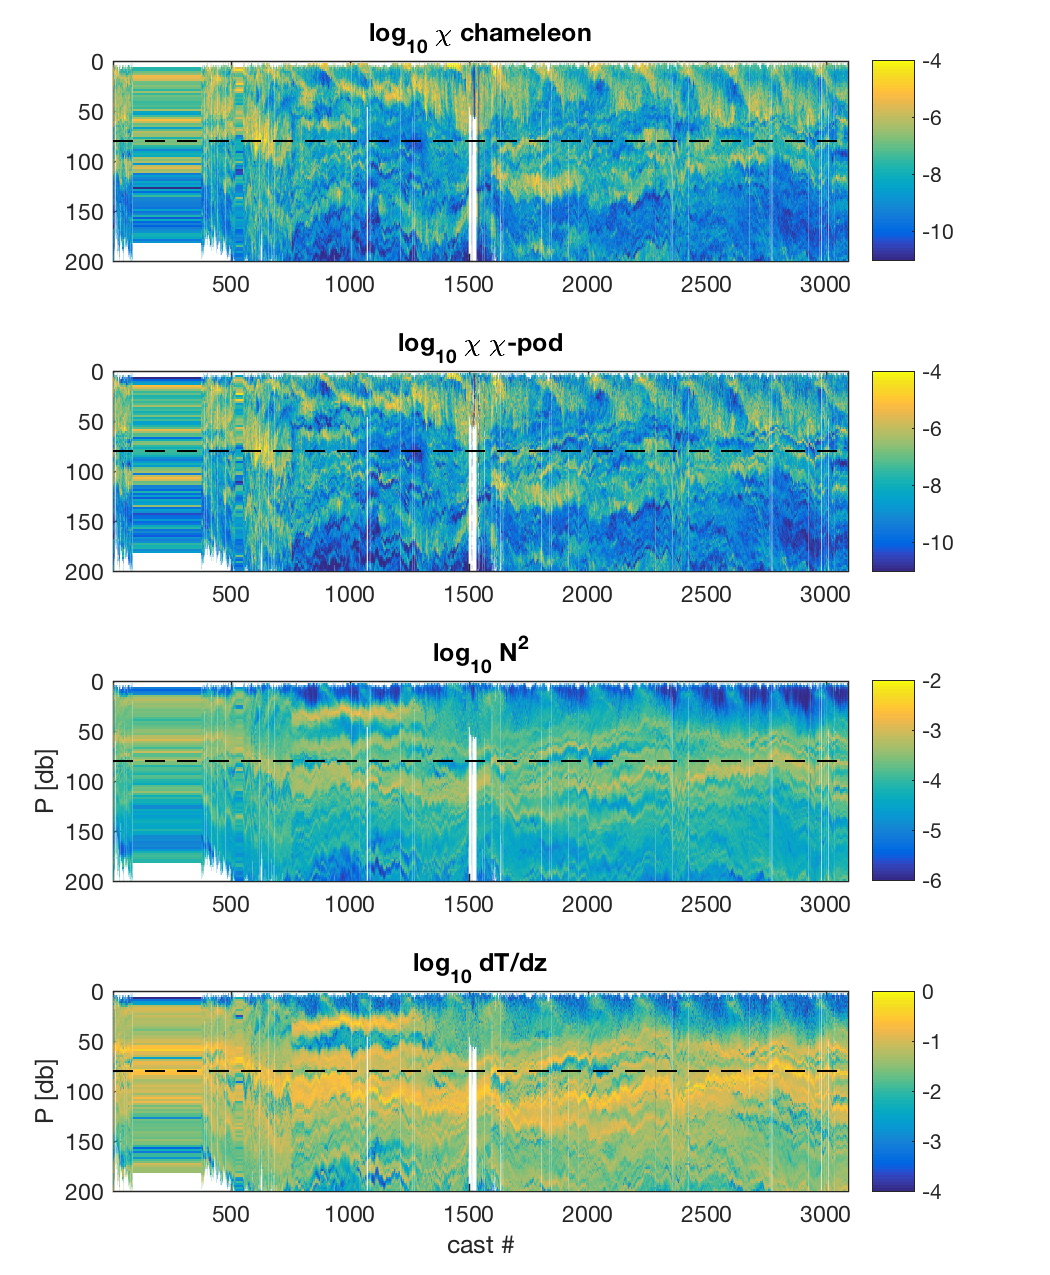
\includegraphics[scale=0.8]{eq14_Pcolor_BothChi_N2_Tz_zsmooth_10_2mbin.png}
\caption{Comparison of $\chi$ from chameleon method and chi-pod method, for EQ14 chameleon profiles. Each profile was averaged in 2m bins.  Values of $\epsion$ below chameleon noise floor (-8.5) have been naned out.}
\label{}
\end{figure}

\begin{figure}[htbp]
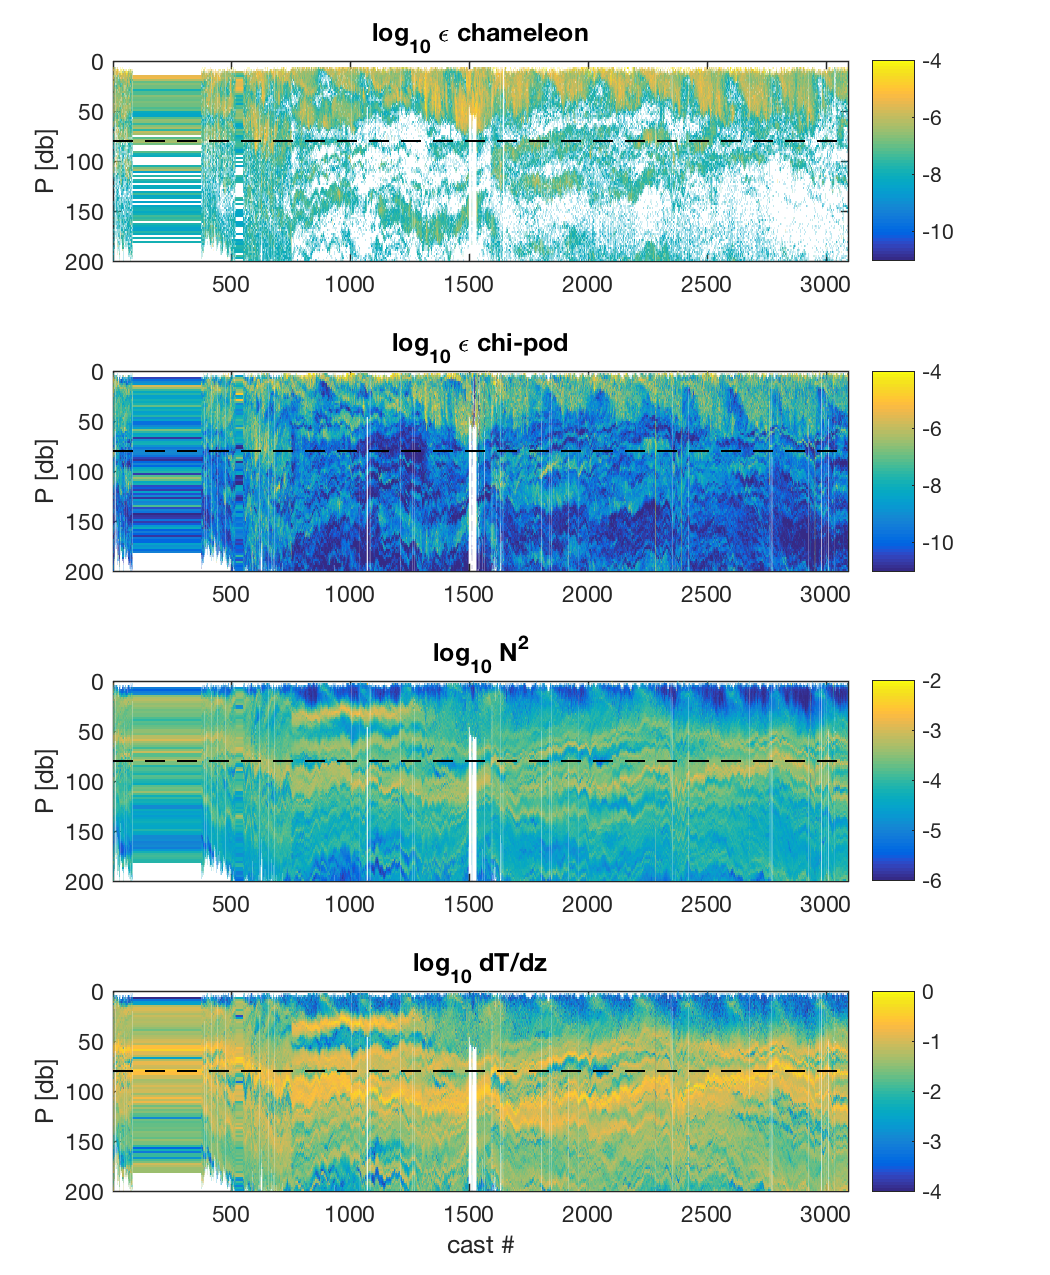
\includegraphics[scale=0.8]{eq14_Pcolor_BothEps_N2_Tz_zsmooth_10_2mbin.png}
\caption{Comparison of $\epsilon$ from chameleon method and chi-pod method, for EQ14 chameleon profiles.}
\label{}
\end{figure}



\clearpage
%~~~~~~~~~
\section{Comparing individual estimates of $\epsilon$}


%\begin{figure}[htbp]
%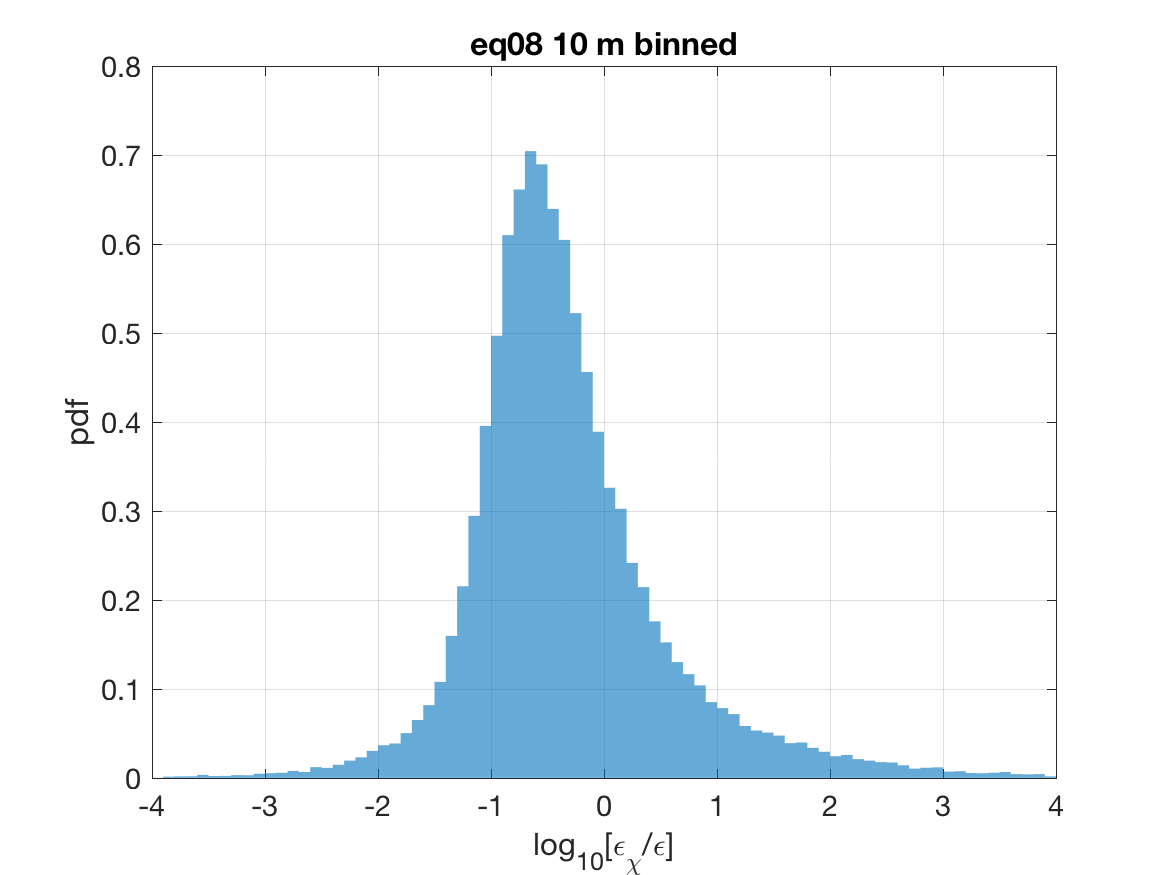
\includegraphics[scale=0.8]{eq08_10mbinned_eps_ratios.png}
%\caption{EQ08: Histogram of the ratio of $\epsilon$ estimates from $\chi$pod method to the chameleon values, for $\chi$pod method applied to 1m binned profiles. Estimates for each profile were averaged in 10m depth bins.}
%\label{epsrathist_eq08}
%\end{figure}


\begin{figure}[htbp]
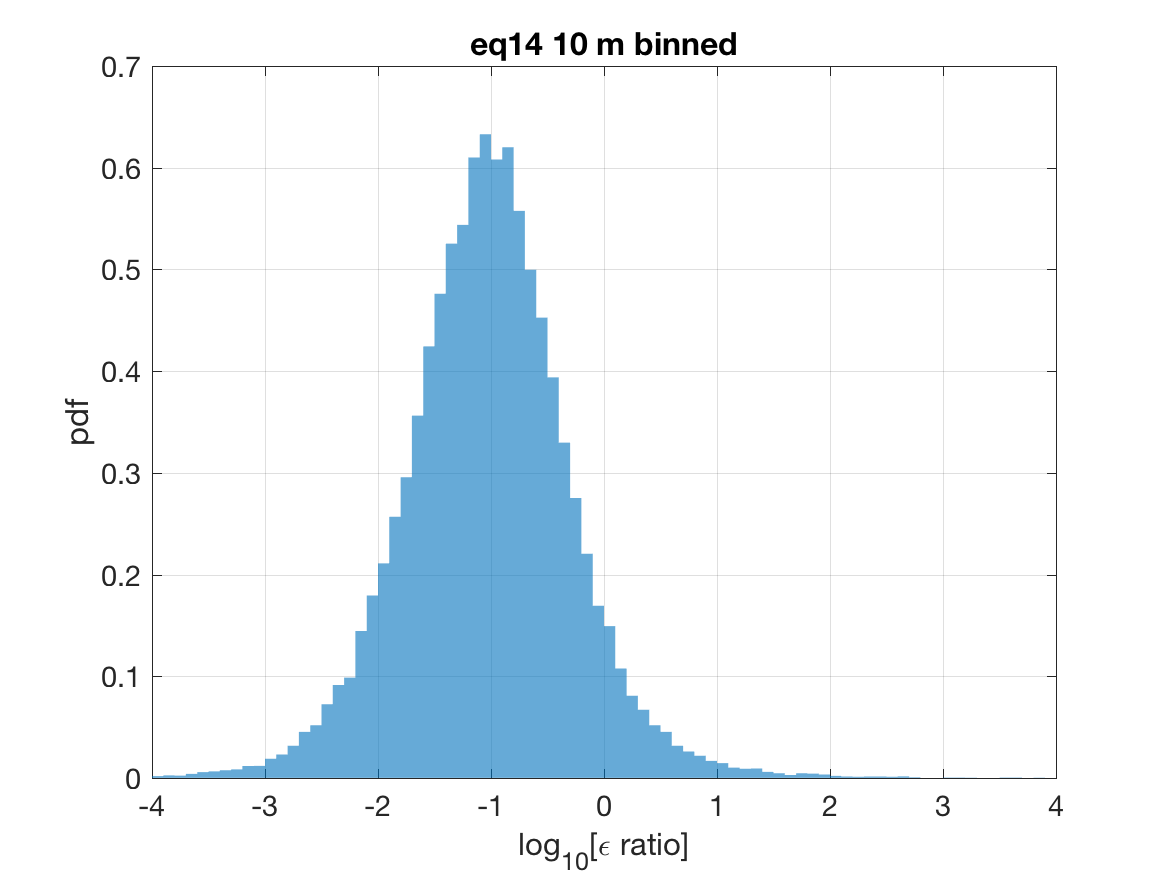
\includegraphics[scale=0.8]{eq14_10mbinned_eps_ratios_Pmin80.png}
\caption{EQ14: Histogram of the ratio of $\epsilon$ estimates from $\chi$pod method to the chameleon values, for $\chi$pod method applied to 1m binned profiles, and applied to just patches. Estimates for each profile were averaged in 10m depth bins.}
\label{epsrathist_eq14}
\end{figure}




\clearpage
%~~~~~~~~~~~~~~~~~~~~~~~~~~~~~
\section{Normalized eps vs chi plots}

Assuming that
\begin{equation}
\gamma=\frac{N^2 \chi}{2\epsilon<T_z>^2}
\end{equation}
, plotting [$\epsilon/N\^2$] vs [$\chi/t_{z}^{2}$] should follow a straight line with slope equal to $1/2\gamma$.

%\begin{figure}[htbp]
%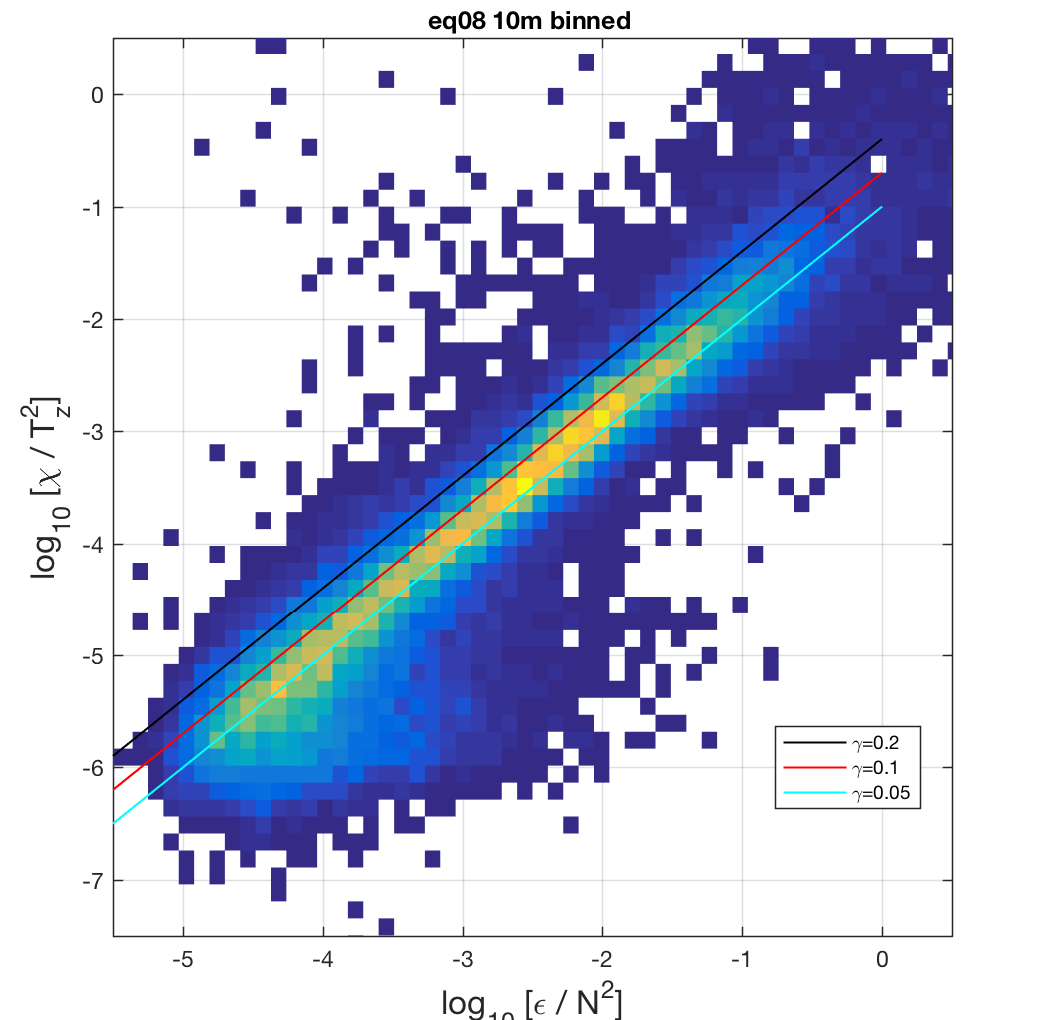
\includegraphics[scale=0.8]{eq08_10mbinned_eps_vs_chi_normalized.png}
%\caption{EQ08: 10m binned  chameleon $\epsilon/N\^2$ vs $\chi/t_{z}^{2}$. Lines show different values of $\gamma$.}
%\label{}
%\end{figure}

%\begin{figure}[htbp]
%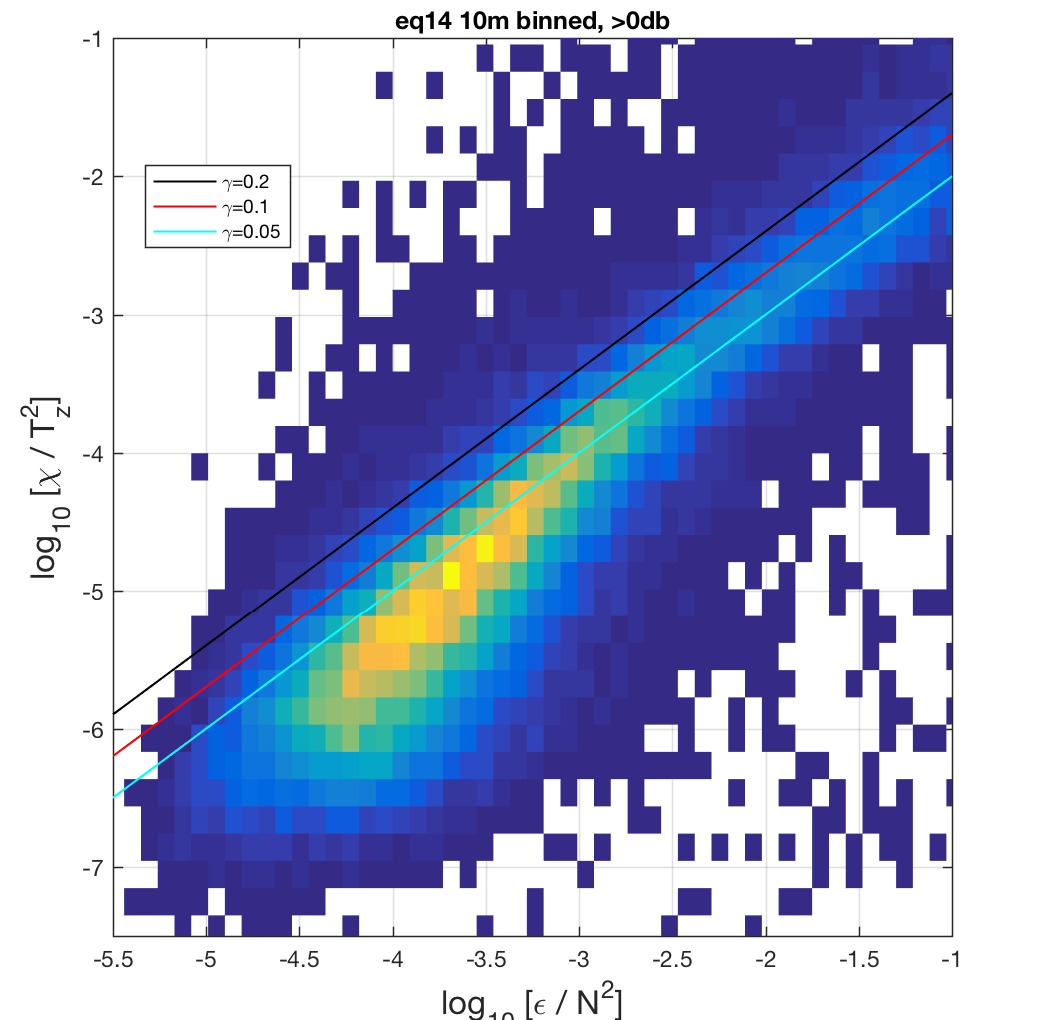
\includegraphics[scale=0.8]{eq14_10mbinned_eps_vs_chi_normalized_Pmin_0.png}
%\caption{EQ14: 10m binned  chameleon $\epsilon/N\^2$ vs $\chi/t_{z}^{2}$ for *ALL depths*. Lines show different values of $\gamma$. Values of $\epsilon$ below noise floor ($log_{10}\epsilon<-8.5$) are discarded also.}
%\label{}
%\end{figure}

\begin{figure}[htbp]
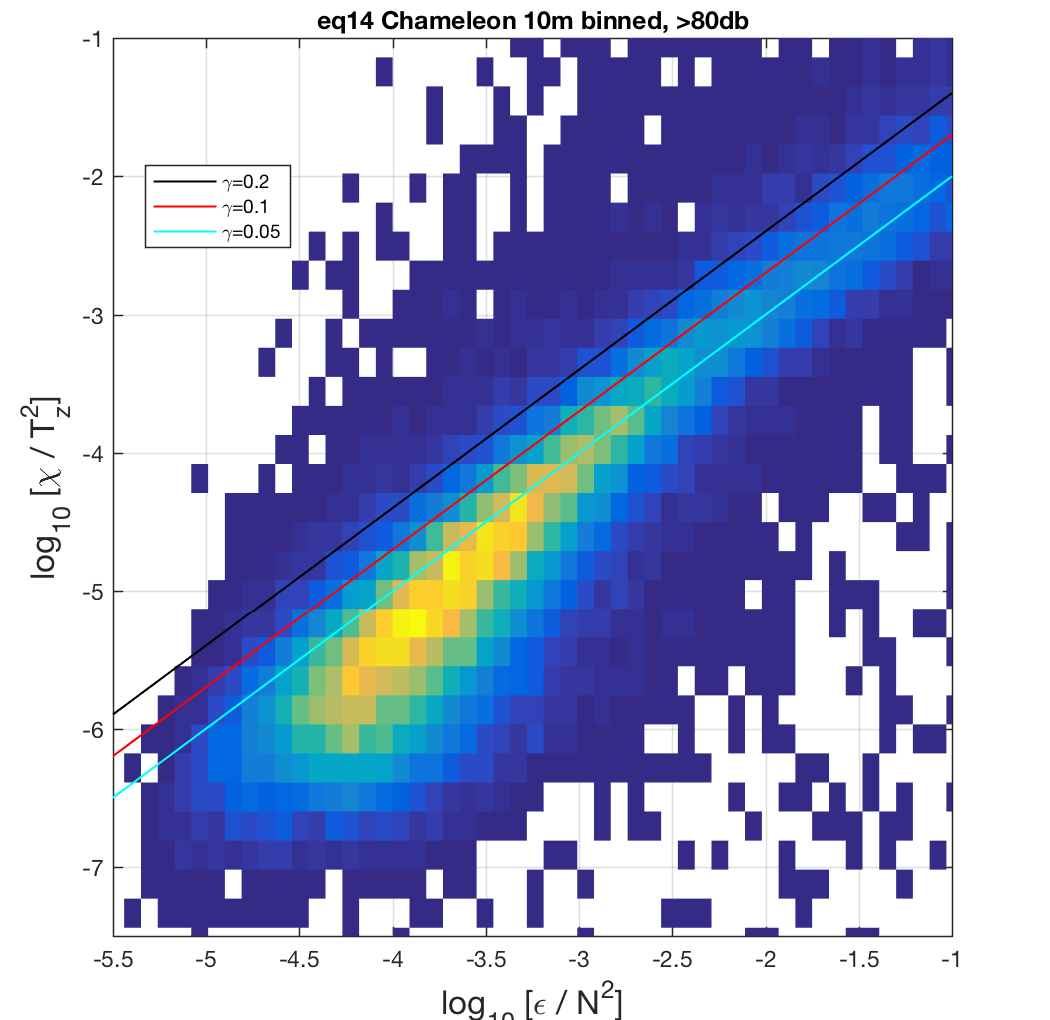
\includegraphics[scale=0.8]{eq14_10mbinned_eps_vs_chi_normalized_Pmin_80.png}
\caption{EQ14: 10m binned  chameleon $\epsilon/N\^2$ vs $\chi/t_{z}^{2}$ for *below 80db*. Lines show different values of $\gamma$. Values of $\epsilon$ below noise floor ($log_{10}\epsilon<-8.5$) are discarded also.}
\label{}
\end{figure}




\clearpage
%~~~~~~~~~
\section{Comparing time-averaged profiles of $\epsilon$}

%Looking at median values and scatterplots might be a little misleading. Maybe what we care about most is the mean profile of $\epsilon$ (or $K_{\rho}$ and $\chi$ (or $K_T$), which are probably dominated by just a small number of large values. 
%
%Figure \ref{epsrathist} shows the ratio of $\epsilon$ estimates (averaged in 10m bins from each profiles) from the $\chi$pod method to chameleon $\epsilon$ values, for both $\chi$pod method applied to 1m binned profiles, and applied to just patches. In such a point-by-point comparsion, the patch estimates have a smaller bias.
%
%
%Figure \ref{eps_prof_comp} shows averaged profiles of $\epsilon$ for several 500-profile chunks of the EQ0-8 data. The average profile of $\chi$pod estimates using 1m bins (`bin') tend to agree well with the chameleon average profile, if $\chi$pod estimates where $log_{10}\epsilon>-4$ are discarded (these are likely bad data due to extremely small dTdz). In fact, the average profile constructed from the binned $\chi$pod estimates tends to agree better than the patch profile.


%\begin{figure}[htbp]
%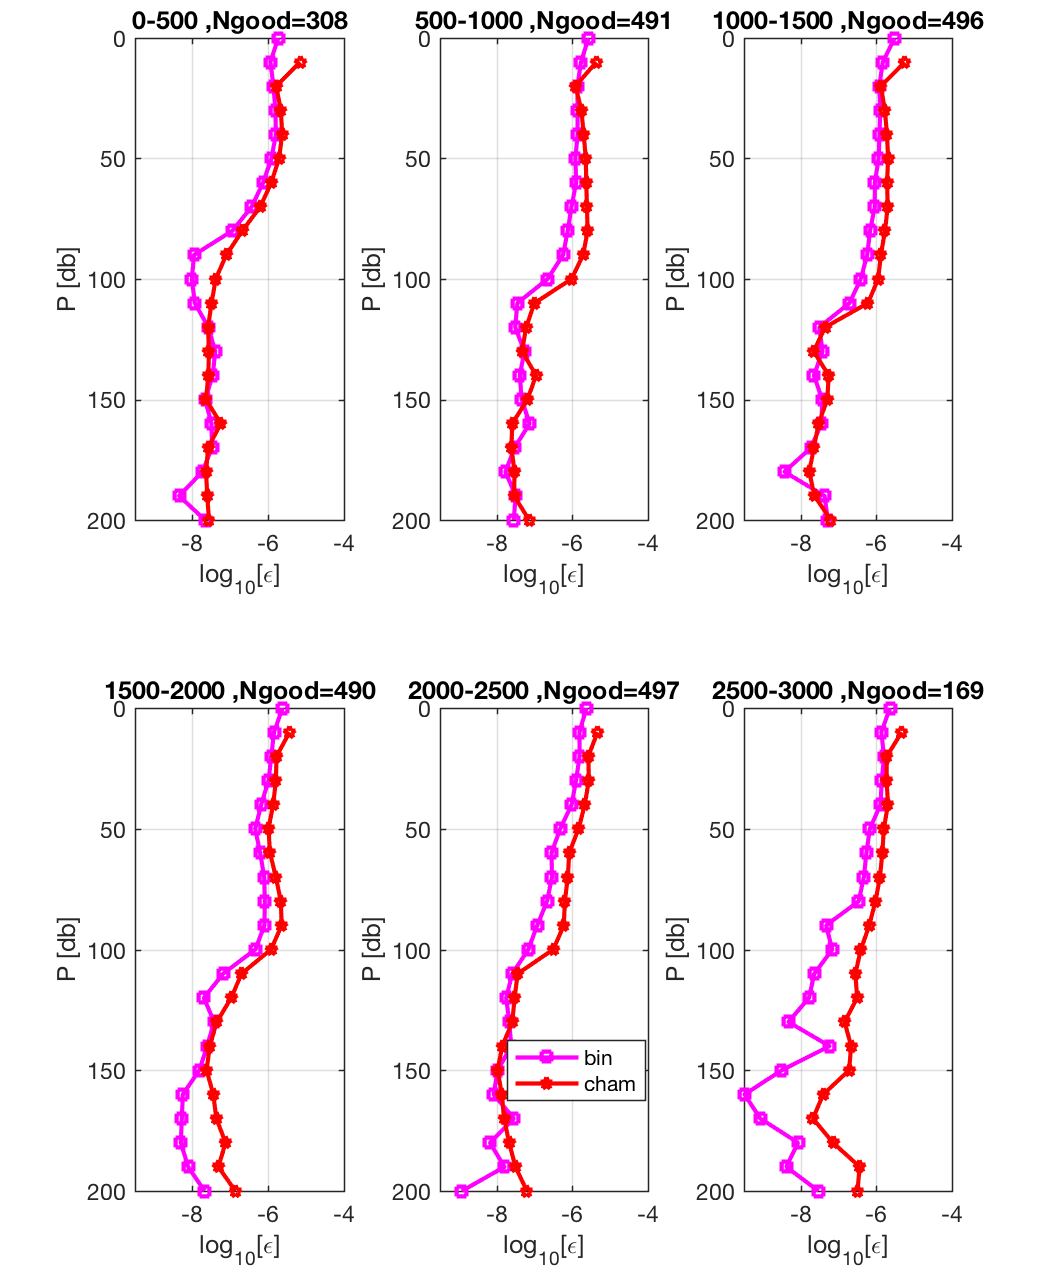
\includegraphics[scale=0.8]{eq08_eps_prof_comparisons.png}
%\caption{EQ08 : Profiles of $\epsilon$, averaged over 500-cast chunks. Different lines are 1m binned Chameleon (`cham'), $\chi$pod method applied over 1m bins (`bin'), and $\chi$pod method appplied to patches (`patch'). *Note $\chi$pod estimates where $log_{10}\epsilon>-4$ are discarded.* Title of each panel gives profile range used, as well as the number of good profiles actually in that range.}
%\label{eps_prof_comp_eq08}
%\end{figure}



\begin{figure}[htbp]
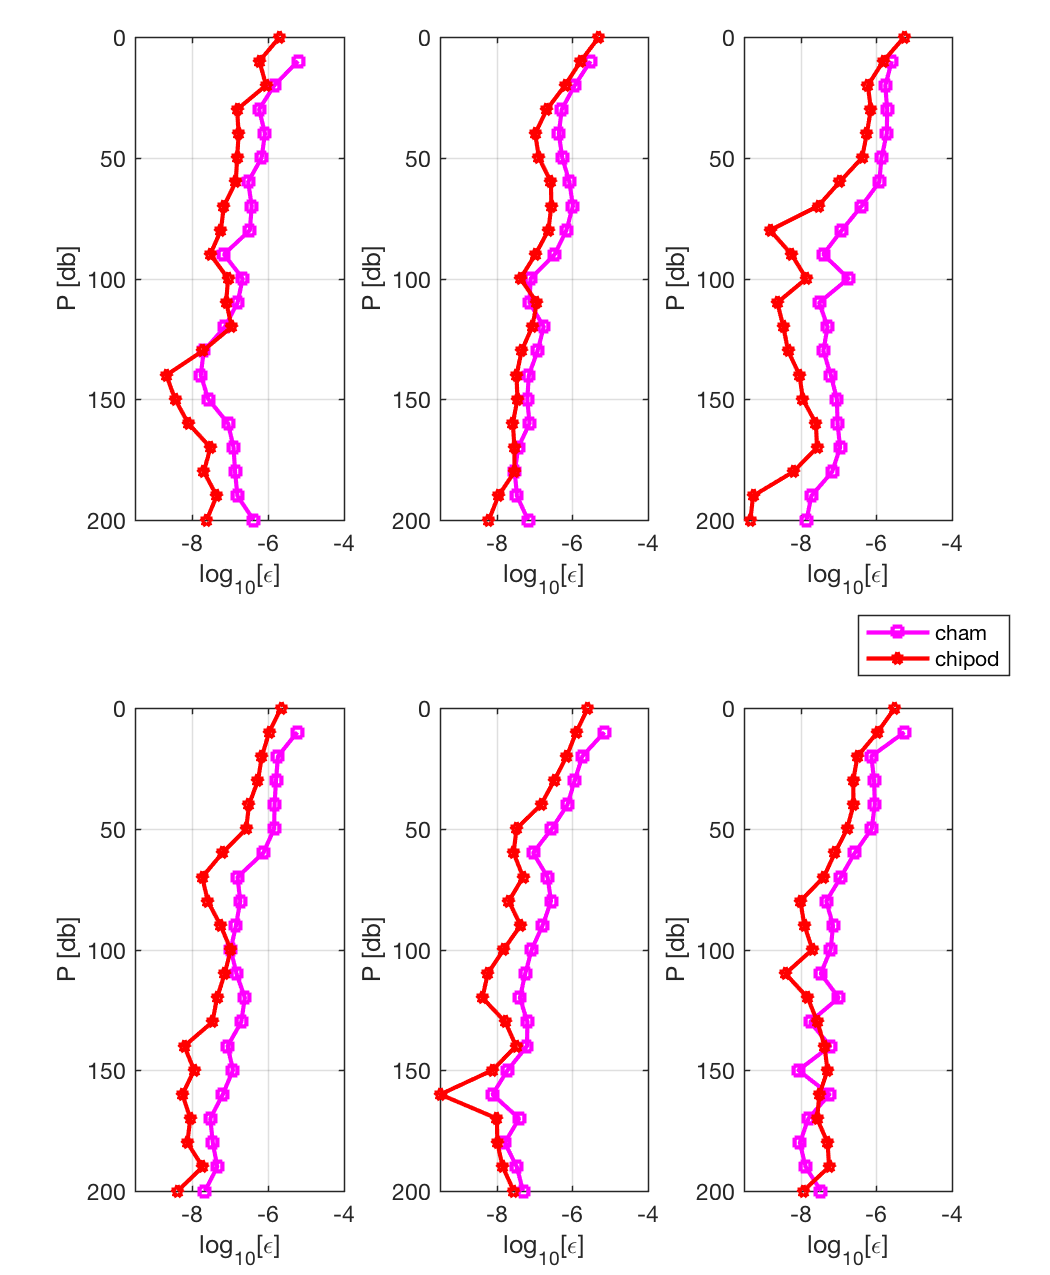
\includegraphics[scale=0.8]{eq14_eps_prof_comparisons_10mbins.png}
\caption{EQ14 : Profiles of $\epsilon$, averaged over 500-cast chunks. Different lines are 1m binned Chameleon (`cham'), $\chi$pod method applied over 1m bins (`bin'), and $\chi$pod method appplied to patches (`patch'). *Note $\chi$pod estimates where $log_{10}\epsilon>-4$ are discarded. Title of each panel gives profile range used, as well as the number of good profiles actually in that range.}
\label{eps_prof_comp_eq14}
\end{figure}


\begin{itemize}
\item Averaging profiles seems to improve the comparisons.
\item $\chi$pod average profiles can be dominated by a few points, which may be spikes/bad data. 
\item What are appropriate thresholds to use? Should I discard chi-pod epsilon lower than -8.5 (same as chameleon?).
\end{itemize}


\begin{figure}[htbp]
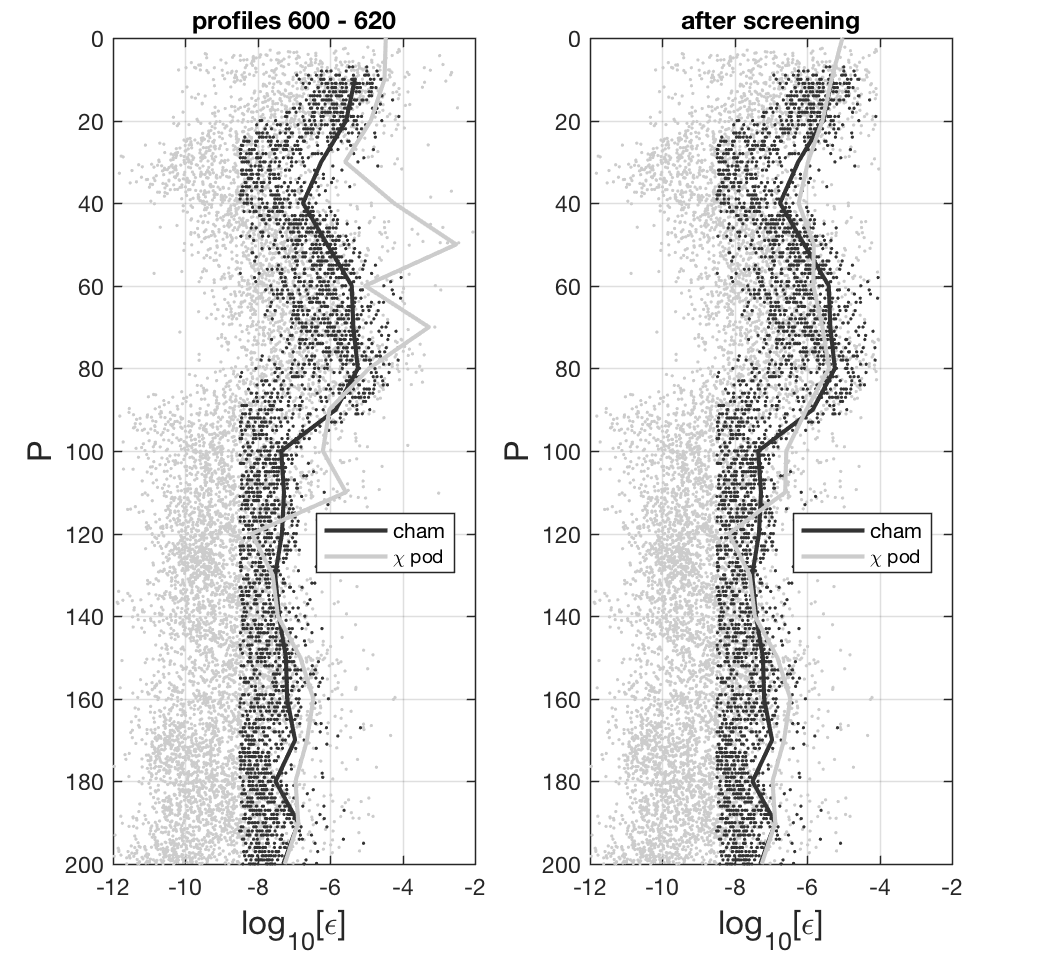
\includegraphics[scale=0.8]{eq14_profiles_600_620_eps_profiles_avg.png}
\caption{}
\label{}
\end{figure}





\clearpage
%~~~~~~~~
\section{Effects of averaging in different-sized depth bins}

I tried making plots of normalized chi vs eps, and scatterplots of chi-pod vs chameleon epsilon, for data averaged in different-sized depth bins (for each profile, not across profiles). They don't seem to change.

\begin{figure}[htbp]
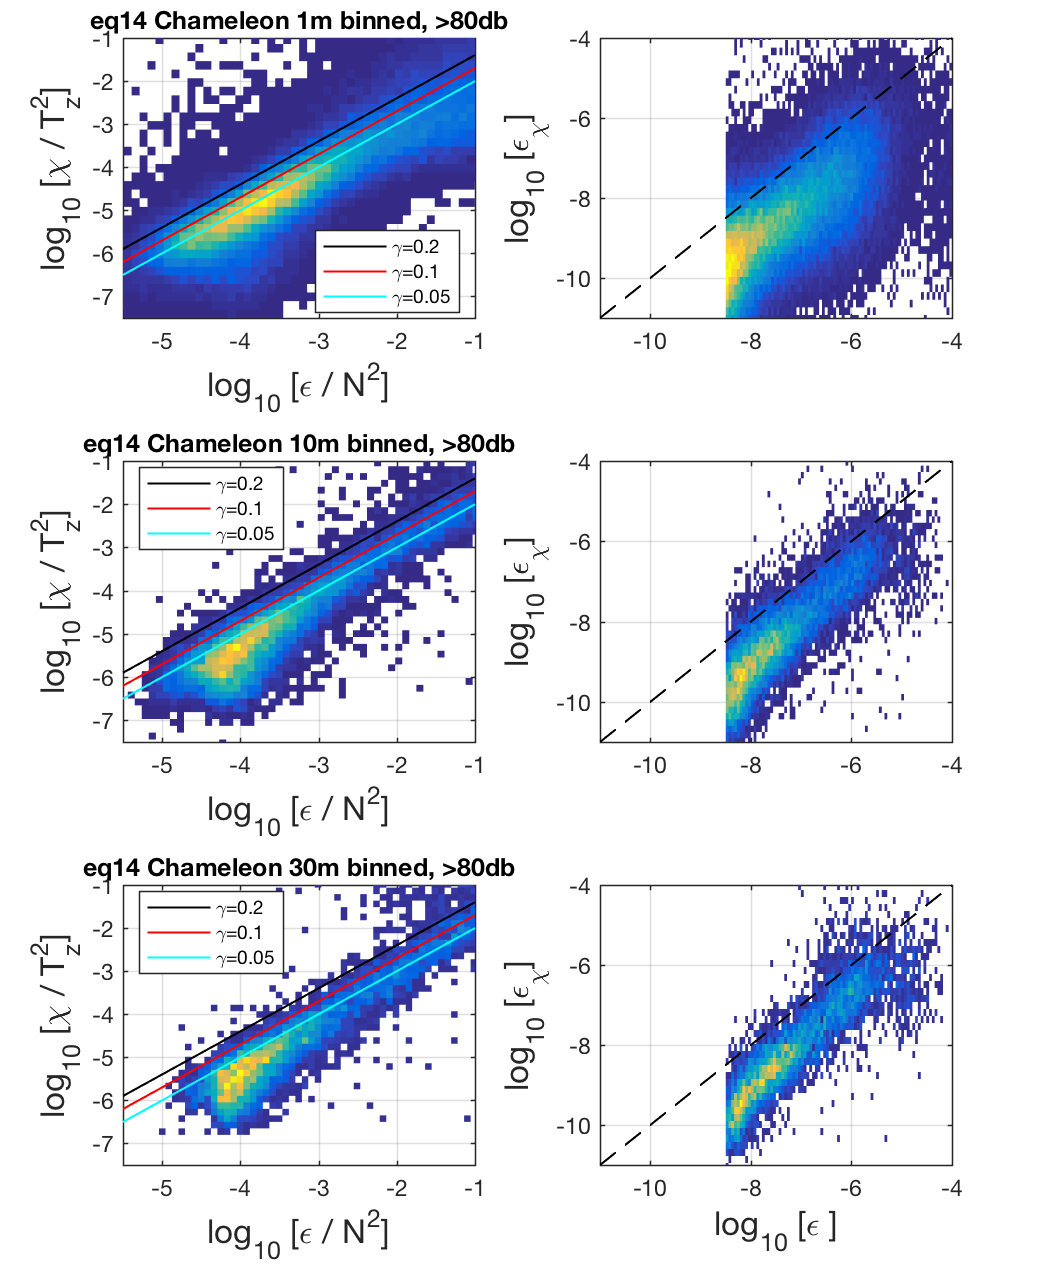
\includegraphics[scale=0.8]{eq14_NormScat_chiVscham_diff_dz.png}
\caption{}
\label{}
\end{figure}




\clearpage
%~~~~~~~~
\section{Effects of averaging different numbers of proifles}

I tried making plots of normalized chi vs eps, and scatterplots of chi-pod vs chameleon epsilon, for data averaged across different numbers of profiles.

\begin{figure}[htbp]
\includegraphics[scale=0.8]{.png}
\caption{}
\label{}
\end{figure}







\clearpage
%~~~~~~~~
\section{$\gamma$ computed from averaged quantities}

If we compute gamma from time-averaged $N^2,T_z,\chi,\epsilon$ do we get $\gamma=0.2$? Estimates from the averaged data are larger (Figures \ref{gambox_eq08},\ref{gambox_eq14}) but still slightly less than 0.2 .

\begin{figure}[htbp]
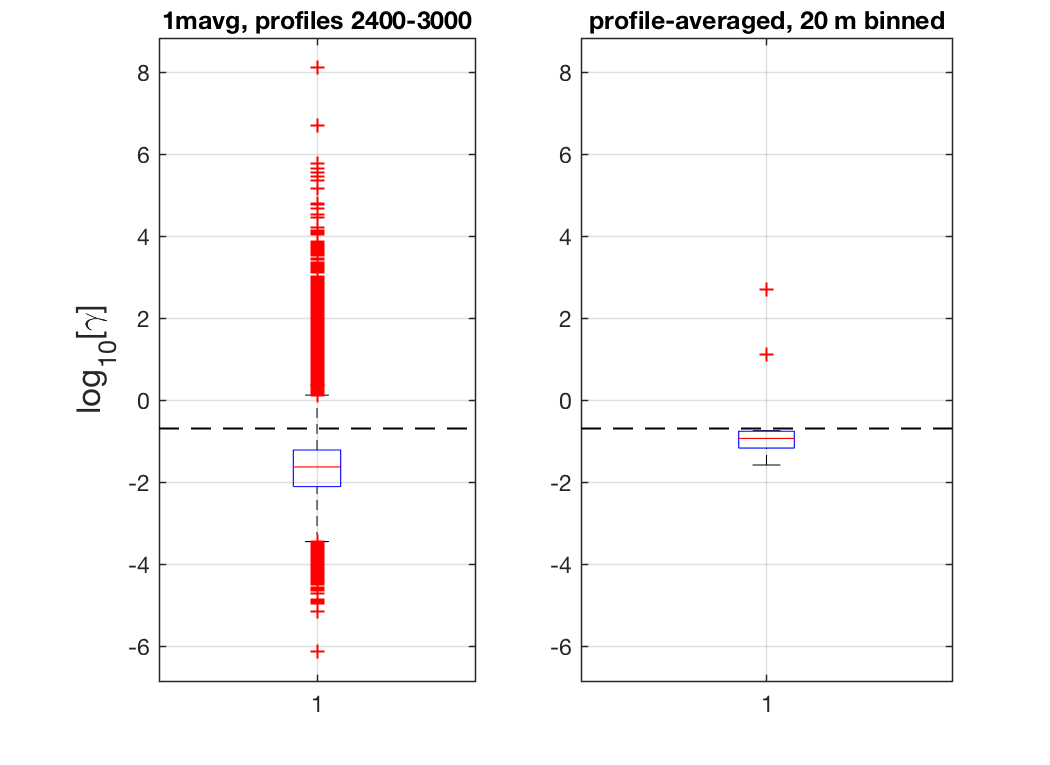
\includegraphics[scale=0.8]{eq14_gamma_point_avg_box_20mbinned.png}
\caption{Boxplots of $log_{10}[\gamma]$ for a set of profiles from EQ14. Left is for all 1m avg data. Right is for data from all profiles averaged in 10m bins. Horizontal dashed line indicates $\gamma=0.2$.}
\label{gambox_eq14}
\end{figure}


\clearpage
%~~~~~~~~
\section{How many profiles need to be averaged to converge?}

Next I wanted to see how many profiles we need to average for the $\chi$pod profile to converge to the chameleon profile. Obviously this will depend on the specific profiles used and the characteristics of the turbulence, but here they seem to converge after about 100-150 profiles. 


%\begin{figure}[htbp]
%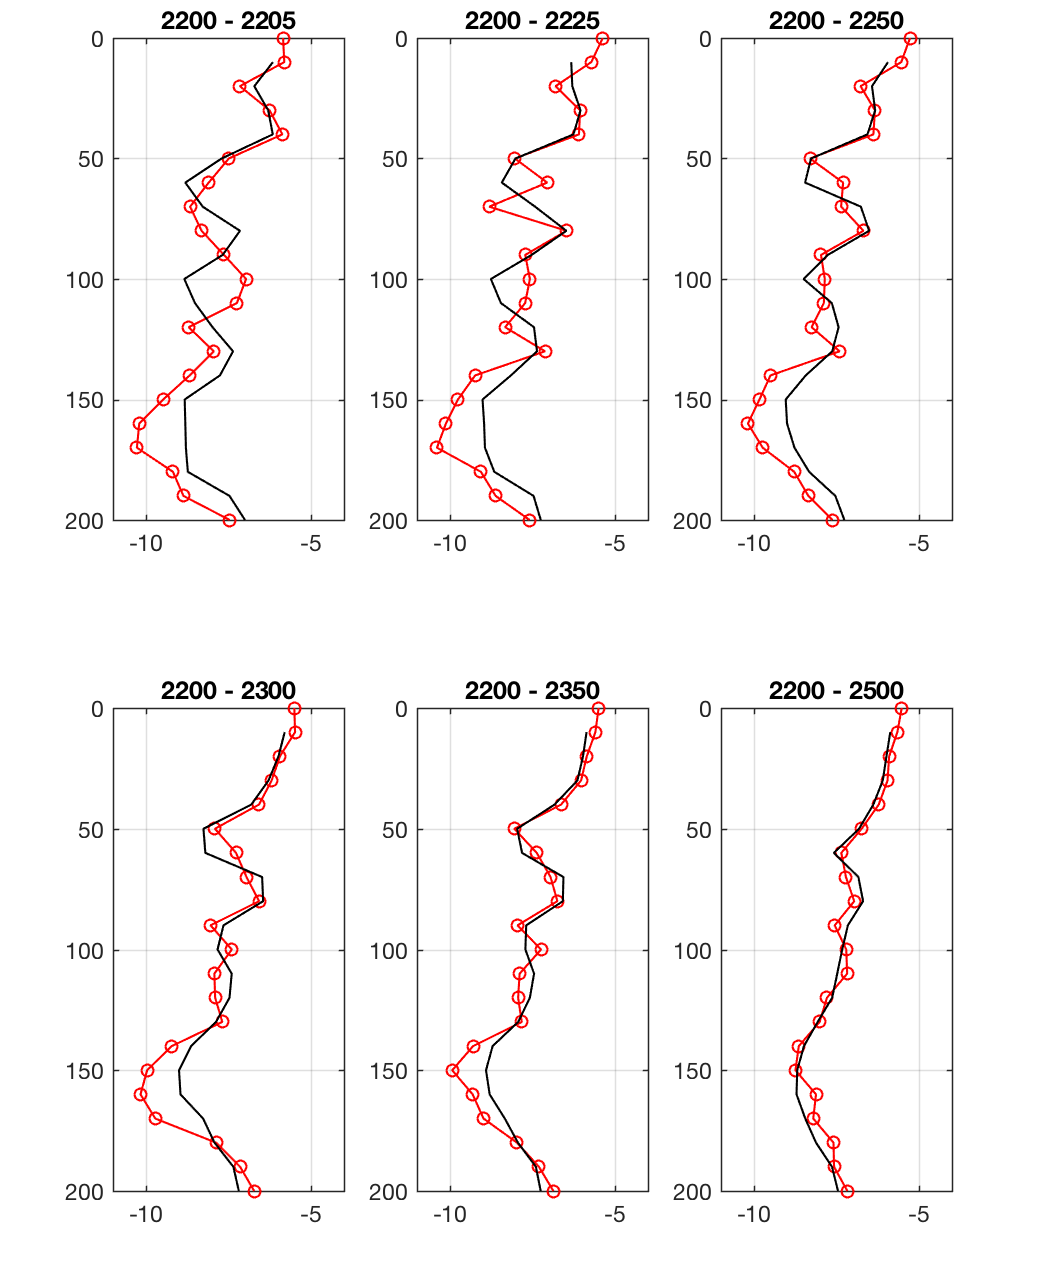
\includegraphics[scale=0.8]{eq14_eps_prof_diffN.png}
%\caption{EQ14: Average profiles of $\epsilon$ from binned $\chi$pod method and chameleon, for different number of profiles (given by title).}
%\label{}
%\end{figure}
%
%
%\begin{figure}[htbp]
%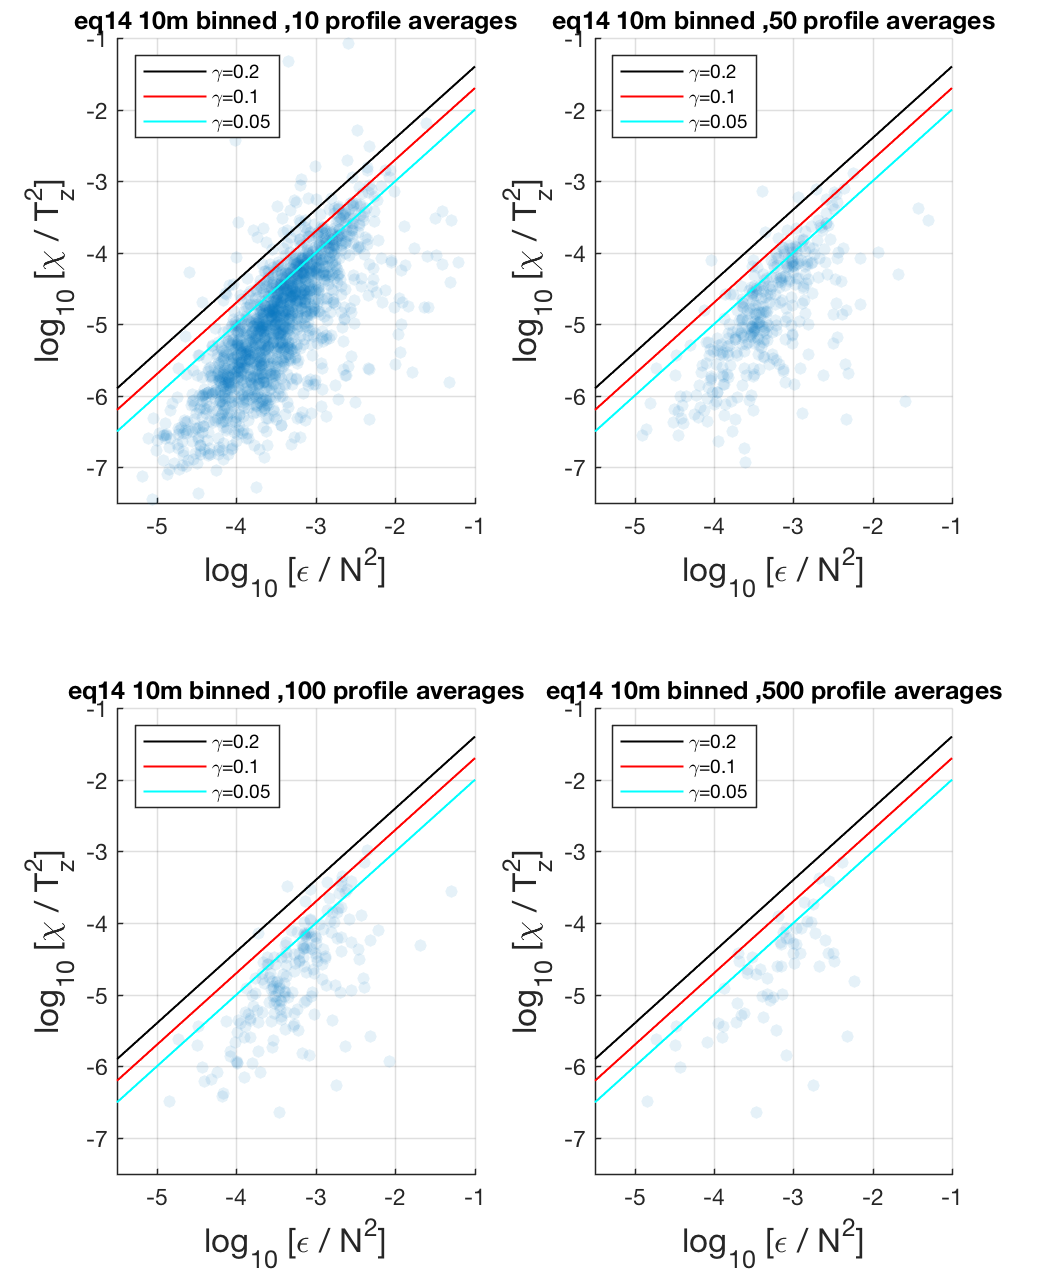
\includegraphics[scale=0.8]{eq14_10mbinned_eps_vs_chi_normalized_diffNprofileAvg_Pmin80.png}
%\caption{EQ14: 10m binned  chameleon $\epsilon/N\^2$ vs $\chi/t_{z}^{2}$, averaged over varying number of profiles. Lines show different values of $\gamma$. Data shallower than 80db have been discarded to avoid mixed layer where night-time convection occurs.}
%\label{}
%\end{figure}






\clearpage
%~~~~~~~~
\section{Summary}

%\begin{itemize}
%\item Inidivudal (and 10m binned) $\chi$pod estimates of $\epsilon$ are biased low compared to Chameleon values.
%\item When many profiles are averaged in 10m bins, the average profiles of $\epsilon$ agree better?.
%\item $\gamma$ computed from averaged (across profiles) $N^2$, $T_z$, $\chi$, and $\epsilon$ is larger, but not quite 0.2 (mean is around 0.1?)
%\item Average profiles seem to converge after about 100 profiles?
%\end{itemize}




\end{document}  


